\documentclass[12pt, A4]{article}
\usepackage{graphicx} % Required for inserting images
\usepackage[english, greek]{babel}
\usepackage[utf8]{inputenc}
\usepackage{wrapfig}
\usepackage{tabularx}
\usepackage{cite}
\usepackage{hyperref}
\usepackage{setspace}
\newcommand{\tl}{\textlatin}
\hypersetup{
    colorlinks=true,
    linkcolor=black,
    filecolor=cyan,      
    urlcolor=blue,
    pdftitle={Overleaf Example},
    pdfpagemode=FullScreen,
}

% Page Margins
\addtolength{\oddsidemargin}{-1in}
\addtolength{\evensidemargin}{-1in}
\addtolength{\textwidth}{1.75in}
\addtolength{\topmargin}{-.875in}
\addtolength{\textheight}{1.75in}

\begin{document}
    \begin{center} % Centering
        \begin{minipage}{10cm}
            
\includegraphics[width=10cm]{logo.jpg}
            \title{\bfseries\fontsize{32}{14}\selectfont Ηθικές Προκλήσεις στην Εποχή των \tl{Big Data} και της Τεχνητής Νοημοσύνης} 
            \author{Ρουμπίνη-Μαρία Αγγουρά ΑΜ:1084634 \and Ιάσονας Παυλόπουλος ΑΜ:1084565}
            \maketitle
        \end{minipage}
    \end{center}
    \newpage
    
    \tableofcontents
    
    \newpage
    
    \section{Υπόμνημα (180 Λέξεις)}
    
    \subsection{Επιλογή Άρθρων}
    \begin{spacing}{1.25}
        \paragraph{Τα επίθετα των μελών της ομάδας, με την σειρά και την μορφή που εκχωρήθηκαν στο πεδίο \tl{String hash} του εργαλείου \tl{Hash Functions} στη σελίδα \tl{fileformat.info}:\\~\\
        ΟΝΟΜΑΤΕΠΩΝΥΜΟ: ΑΓΓΟΥΡΑ ΠΑΥΛΟΠΟΥΛΟΣ \newline
        \tl{SHA-1:}\hspace{3.9cm}\tl{43cf85727d585def0aedb8c329ae0ab9e9ac25a4} \newline
        Διακριτά ψηφία:\hspace{1.9cm}4, 3, 8, 5, 7, 2}
        
        \paragraph{Τα άρθρα της κατηγορίας \tl{Ethics} που προέκυψαν μετά από αυτή τη διαδικασία είναι:\\}
    
        \begin{center}
            \begin{tabular}{ |c|c| }
                 \hline
                 4 & \tl{What is Überveillance? (And What Should Be Done About It?)}\\
                 \hline
                 3 & \tl{Mimetic Models: Ethical Implications of AI that Acts Like You}\\
                 \hline
                 8 & \tl{Algorithmic amplification of politics on Twitter}\\
                 \hline
                 5 & \tl{Ethics for Big Data and Analytics}\\
                 \hline
                 7 & \tl{Social ethics in Internet of Things:An outline and review}\\
                 \hline
                 2 & \tl{Critiquing Big Data: Politics, Ethics, Epistemology}\\ 
                 \hline
            \end{tabular}
        \end{center}
    \end{spacing}

    \subsection{Ομάδα}
        \paragraph{Στο πλαίσιο αυτής της εργασίας, τα μέλη είχαμε άψογη συνεργασία, συνεχή επικοινωνία και υψηλή αποδοτικότητα. Αρχίσαμε την εργασία, έχοντας ήδη αποφασίσει για την επιλογή της κατηγορίας των \tl{Ethics}, αφού ήταν το θέμα που μας κινούσε το ενδιαφέρον περισσότερο, δημιουργήσαμε ένα κοινό \tl{Google Docs} έγγραφο. Έτσι, καθώς παράλληλα γινόταν η ανάγνωση και κατανόηση των άρθρων που μας ανατέθηκαν, σημειώναμε τα κύρια στοιχεία τους στο παραπάνω έγγραφο. Έχοντας μια σφαιρική άποψη πλέον συλλογικά για όλα τα άρθρα, προχωρήσαμε στην επιλογή των τεσσάρων που είχαν την πιο ισχυρή σύνδεση και σαφήνεια. Στην συνέχεια, αρχίσαμε την συγγραφή της εργασίας σε \tl{Latex}, στην οποία και οι δύο πληκτρολογούσαμε ταυτόχρονα μέσω της πλατφόρμας \tl{Overleaf}. Έχοντας δημιουργήσει το βασικό \tl{Layout} της εργασίας, προχωρήσαμε στην συγγραφή της Περίληψης, της Βιβλιογραφικής Παρουσίασης, της Βιβλιογραφίας, της Παρουσίασης σε \tl{PowerPoint} και την λήψη του βίντεο. Τα παραπάνω βήματα πραγματοποιήθηκαν από κοινού με τον ίδιο αριθμό ωρών εργασίας, με αποτέλεσμα να αποκτηθεί η απαραίτητη εμπειρία σε όλους τους τομείς που απασχολεί αυτή η εργασία και από τα δύο μέλη της ομάδας μας.}
    \newpage

    \section{Περίληψη (167 Λέξεις)}
    \paragraph{Η εφαρμογή τεχνολογιών, στην καθημερινότητα μας, όπως η τεχνητή νοημοσύνη και τα \tl{Big Data}, παίζουν σημαντικό ρόλο στην διαμόρφωση της σημερινής κοινωνίας. Ωστόσο, ο αποκλειστικός έλεγχος και η χρήση τους από εταιρίες και οργανισμούς, η σκόπιμη έλλειψη ενημέρωσης σχετικά με αυτές και τους κινδύνους που επιφυλάσσουν και ο ενθουσιασμός των χρηστών με την επαφή τους με αυτές, θίγουν καινούρια ηθικά ζητήματα. Στα άρθρα που θα παρουσιάσουμε, οι συγγραφείς περιγράφουν αυτά τα προβλήματα και τα αναλύουν. Σκοπός των άρθρων αυτών είναι να αποδείξουν πως είναι ανάγκη να γίνει επανεξέταση των ηθικών κανόνων που ήδη υπάρχουν και η δημιουργία νέων για κάθε νέο τεχνολογικό επίτευγμα. Έπειτα, προτείνουν πιθανές λύσεις, όπως τον περιορισμό της ανεξέλεγκτης χρήσης τους, την πρόσβαση των ανθρώπων στα προσωπικά τους δεδομένα και την γνωστοποίηση των τεχνικών που χρησιμοποιούνται για την επεξεργασία αυτών. Τέλος, τονίζουν πως ακόμα και η καινούρια νομοθεσία, θα πρέπει συνεχώς να ενημερώνεται, αφού οι τεχνολογίες για τις οποίες γίνεται λόγος, είναι σε διαρκή εξέλιξη και δεν είναι βέβαιο τι κινδύνους μπορεί να κρύβουν.}
    \newpage

    \section{Βιβλιογραφική Παρουσίαση (931 Λέξεις)}
    \paragraph{Την τελευταία δεκαετία, έχει παρατηρηθεί ραγδαία εξέλιξη σε πολλούς διαφορετικούς τομείς της τεχνολογίας. Σαν συνέπεια, πολλοί επιστήμονες προβληματίζονται για τα ηθικά διλήμματα που τίθονται και τις προκλήσεις που εμφανίζονται, όταν οι νέες αυτές τεχνολογίες συλλέγουν, επεξεργάζονται, ερμηνεύουν και χρησιμοποιούν μεγάλο πλήθος προσωπικών δεδομένων. Είναι ηθική η μαζική συλλογή προσωπικών δεδομένων? Πώς μπορεί να επηρεάσει η χρήση των τεχνολογιών \tl{AI} την κοινωνία αλλά και την καθημερινοτητά μας?}
    
    \paragraph{Όπως αναφέρουν και στο άρθρο τους οι \tl{Kate Crawford, Kate Milner} και η \tl{Mary L. Gray} \cite{article2}, τα \tl{Big Data} αντιμετωπίζουν ως φαινόμενο αρκετά ηθικά διλλήματα. 
    Υποστηρίζεται αρχικά, πως οι άνθρωποι, ενθουσιασμένοι από τα οφέλη που έχουν πειστεί ότι τα \tl{Big Data} θα τους προσφέρουν, μοιράζονται τα δεδομένα τους χωρίς δεύτερη σκέψη, ξεχνώντας μια βασική αρχή της κοινωνίας, το γεγονός ότι ατομικές πράξεις δεν μπορούν ποτέ να αναπαραστήσουν τις πολύπλοκες δυναμικές που υπάρχουν μέσα σε μία κοινωνία. Όπως αναφέρεται στο άρθρο, υπάρχει ένας μεγάλος διαχωρισμός ανάμεσα σε εμάς και τα δεδομένα μας. Αυτό οφείλεται στο ότι συνήθως δεν έχουμε πρόσβαση σε αυτά, αλλά ούτε και τις απαραίτητες γνώσεις για να τα κατανοήσουμε και να τα ερμηνεύσουμε. Αυτό έχει ως αποτέλεσμα, λίγοι τελικά να παίρνουν αποφάσεις που αφορούν πολλούς. Όμως, και η ερμηνεία των δεδομένων ως έχει, δημιουργεί ένα σημαντικό ηθικό πρόβλημα. Από την στιγμή που κανένας δεν μπορεί να είναι πλήρως αντικειμενικός, κάθε άτομο μπορεί να τα ερμηνεύσει και με διαφορετικό τρόπο, βγάζοντας ένα εντελώς διαφορετικό συμπεράσμα. Είναι προφανές, λοιπόν, πως η ανάγκη για νέους κανόνες είναι μεγάλη. Αυτό τονίζει και στο άρθρο του ο \tl{Daniel E. O’Leary} \cite{article5}. Πιο συγκεκριμένα, σχολιάζει πως τα \tl{Big Data} ακολουθούν ακόμα τη δεοντολογία που δημιουργήθηκε για τους υπολογιστές, και υποστηρίζει πως αυτό δεν είναι αρκετό. Πιστεύει, πως επειδή οι λόγοι για την ύπαρξη κανόνων στην κάθε περίπτωση είναι θεμελιωδώς διαφορετικοί, θα πρέπει να αναπτυχθεί νέα δεοντολογία που θα αφορά συγκεκριμένα το κομμάτι των \tl{Big Data}.}

    \paragraph{Ένα ακόμα φαινόμενο που έχει προκύψει από την εξέλιξη της τεχνολογίας και την πρόσβαση σε \tl{Big Data} μόνο από μεγάλους οργανισμούς και επιχειρήσεις, είναι το \tl{Überveillance}, το οποίο πραγματεύεται ο \tl{Roger Clarke} \cite{article4}, στο άρθρο του. Ειδικότερα, με την διαρκή παρακολούθηση των πολιτών, η κύρια ανησυχία του συγγραφέα, είναι η θυσία της ιδιωτικότητας, της αυτονομίας και των πολιτικών ελευθεριών, στο όνομα της ασφάλειας, χωρίς να παραβλέπονται τα προβλήματα που εντοπίστηκαν παραπάνω σχετικά με την επεξεργασία των προσωπικών δεδομένων. Επομένως, ο συγγραφέας, προτείνει συγκεκριμένα μέτρα τα οποία μοιάζουν αναγκαία για να διατηρηθεί η ασφάλεια της κοινωνίας, χωρίς αυτή να ελέγχεται από συγκεκριμένες μονάδες. Για παράδειγμα, απαραίτητη φαίνεται η αιτιολόγηση των μέτρων που λαμβάνονται σχετικά με την ασφάλεια και η δυνατότητα αξιολόγησής τους από το κοινό, καθώς έτσι δημιουργείται μια σχέση εμπιστοσύνης μεταξύ των εποπτών και το εποπτευόμενων. Ακόμη, ιδιαίτερα σημαντική είναι και η δυνατότητα πρόσβασης στα προσωπικά δεδομένα παρακολούθησης, αφού με αυτόν τον τρόπο εξασφαλίζεται η επαλήθευση της αντικειμενικότητας των αποφάσεων που λαμβάνονται με βάση αυτά.}

    \paragraph{Τέλος, θα θέλαμε να θίξουμε ένα ακόμα θέμα που απαιτεί ιδιαίτερη προσοχή και αναλύουν στο άρθρο τους οι \tl{Reid McIlroy-Young, Jon Kleinberg, Siddhartha Sen, Solon Barocas} και \tl{Ashton Anderson} \cite{article3}, την δημιουργία των \tl{mimetic models}. Τα \tl{mimetic models} αποτελούν έναν αλγόριθμο ο οποίος έχει σκοπό να μιμηθεί αλλά και να προβλέψει συμπεριφορές ανθρώπων σε μελλοντικά σενάρια ακόμα και αν δεν έχουν βρεθεί ξανά σε παρόμοια κατάσταση. Έχουν πολλούς τομείς στους οποίους μπορούν να χρησιμοποιηθούν, όπως στην προετοιμασία για συνεντεύξεις, δημιουργώντας ένα \tl{mimetic model} του ατόμου που πραγματοποιεί την συνέντεξη, ή σε διαγωνισμούς, κατασκευάζοντας ένα μοντέλο το οποίο θα μιμείται τον αντίπαλο. Αντίστοιχα, μπορούν να υλοποιηθούν \tl{mimetic models} με βελτιωμένα χαρακτηριστικά αντικαθιστώντας εργαζόμενους σε μία επιχείρηση. Ακόμα, με τα \tl{mimetic models}, γίνεται πολύ πιο εύκολη η εξαπάτηση και η χειραγώγηση των άλλων ανθρώπων, από αυτούς που τα διαθέτουν. Όλοι αυτοί οι τρόποι χρήσης τους, δημιουργούν στον αρθρογράφο αρκετές απορίες, όπως το αν θα μειωθεί η αξία του ίδιου του ατόμου αν υπάρχει ένας τέτοιος αλγόριθμος, ή το πόσο αξιόπιστο είναι όντως ένα τέτοιο μοντέλο και αν θα πρέπει να διατίθεται σε όλους.}

    \paragraph{Τέλος, μπορούν να μελετηθούν και άλλες ενδιαφέρουσες πηγές για τα παραπάνω ζητήματα που απασχολούν την σημερινή κοινωνία: \cite{article1}, \cite{article6}, \cite{article7}, \cite{article8}, \cite{article9}, \cite{article10}, \cite{article11}\\}
    
    \paragraph{\underline{Κριτική συζήτηση με το \tl{ChatGPT}}}
    \paragraph{-Ποια είναι τα βασικά σημεία του άρθρου \tl{Mimetic Models: Ethical Implications of AI that Acts Like You}?\\~\\
    -Το άρθρο \tl{"Mimetic Models: Ethical Implications of AI that Acts Like You"} παρουσιάζει μια μελέτη για τις επιπτώσεις της τεχνολογίας της τεχνητής νοημοσύνης (AI) που δημιουργεί μοντέλα μιμητικής μάθησης (\tl{mimetic learning}) και έχει ως στόχο την αναπαραγωγή του ανθρώπινου συμπεριφοράς στην κοινωνία. Οι συγγραφείς εξετάζουν την ηθική πτυχή της χρήσης τέτοιων συστημάτων, καθώς επηρεάζουν τον τρόπο με τον οποίο αλληλεπιδρούμε με τα υπολογιστικά συστήματα, καθώς και την προστασία της ιδιωτικής ζωής και την ανθρώπινη αξιοπρέπεια. Στη μελέτη παρουσιάζονται διάφορες περιπτώσεις με χρήση μοντέλων μιμητικής μάθησης, όπως η απομίμηση της γλώσσας και η αναπαραγωγή συμπεριφοράς στο διαδίκτυο, και αναλύονται οι επιπτώσεις τους στην κοινωνία. Τέλος, παρουσιάζονται προτάσεις για τη βελτίωση της ανθρωπότητας των μοντέλων μιμητικής μάθησης και την αντιμετώπιση των ηθικών προκλήσεων που προκύπτουν από τη χρήση τους.\\~\\
    Όπως φαίνεται από τον παραπάνω διάλογο, το \tl{ChatGPT} αναφέρει ως βασικά σημεία του κειμένου, θέματα που δεν υπάρχουν στο κείμενο. Για παράδειγμα, γράφει πως στο κείμενο παρουσιάζονται προτάσεις για την βελτίωση της ανθρωπότητας των μοντέλων μιμητικής μάθησης, αλλά στο κέιμενο δεν αναγράφεται κάτι σχετικό. Είναι εύκολο να συμπεράνουμε λοιπόν, πως ενώ δίνει μια απάντηση σωστά δομημένη η οποία εκ πρώτης όψης φαίνεται να είναι ορθή, τελικά έχει σημαντικά λάθη.}
    
    \paragraph{\underline{Συζήτηση}}
    \paragraph{Συμπερασματικά, συμφωνούμε με τους συγγραφείς και πιστεύουμε πως για την ομαλή λειτουργία της κοινωνίας μας αλλά και για την εξασφάλιση της δικαιοσύνης και της αντικειμενικότητας, θα πρέπει να δοθεί η απαραίτητη προσοχή στα παραπάνω θέματα, και να δημιουργηθούν καινούριοι ηθικοί κανόνες, ειδικά προσαρμοσμένοι σε αυτά.}
    \newpage
    
    \section{Βιβλιογραφία}
    
    \bibliographystyle{IEEEtran}
    \bibliography{main.bib}
    \newpage
    
    \section{Βιογραφικά (211 Λέξεις)}
    
    \paragraph{Η Ρουμπίνη Μαρία Αγγουρά είναι φοιτήτρια του τμήματος Μηχανικών Η/Υ του Πανεπιστημίου Πατρών και διανύει το 3ο έτος των σπουδών της. Είναι μια φοιτήτρια προσηλωμένη στον στόχο της, γεμάτη δημιουργικότητα και πρωτοποριακές ιδέες που μπορούν να δώσουν στον χώρο της τεχνολογίας μια νέα πνοή. Έχει συμμετάσχει μεταξύ άλλων, σε διαγωνισμούς ρομποτικής, στατιστικής και έχει ταξιδέψει στην Ισπανία και Ιταλία μέσω προγράμματος \tl{Erasmus}+. Στον ελεύθερο της χρόνο, ασχολείται με την υποκριτική και δεν χάνει ποτέ την ευκαιρία να διαβάσει ένα καλό βιβλίο και να πάει μια βόλτα. Έχει διαπιστώσει πως μόνο καλλιεργώντας όλες τις πτυχές της προσωπικότητάς του, μπορεί κανείς να είναι αποτελεσματικός, αποδοτικός και ευτυχισμένος.\\}
    
    \begin{wrapfigure}{l}{0.27\textwidth}
	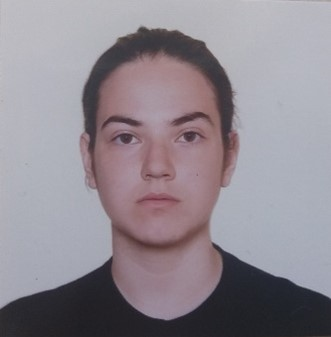
\includegraphics[width=\linewidth]{Bio/bio1.jpg}
    \end{wrapfigure}
    
    \paragraph{Ο Ιάσονας Παυλόπουλος, γεννημένος στον Πειραιά, είναι 3οετής φοιτητής του τμήματος Μηχανικών Η/Υ και έχει επιδείξει μεγάλη αφοσίωση στον τομέα της τεχνολογίας. Έχοντας ένα πλούσιο γνωστικό υπόβαθρο στον τομέα του προγραμματισμού, της σχεδίασης κυκλωμάτων και της ανάπτυξης αλγορίθμων, με πάθος προς την επίλυση προβλημάτων, έχει αποδείξει με την ακαδημαϊκή του πορεία, αλλά και σε διαγωνισμούς προγραμματισμού και ρομποτικής όπως \tl{Zero Robotics}, \tl{WRO Hellas} και \tl{SNF Hackathon}, την αδιάλειπτη ανάπτυξή του στον τομέα. Μετά την αποφοίτηση, στόχος του είναι να ακολουθήσει μία καριέρα στην ανάπτυξη λογισμικού με φιλοδοξία να συμβάλει σημαντικά στον κλάδο για τα επόμενα χρόνια.}
    
    \begin{wrapfigure}{l}{0.27\textwidth}
	
\includegraphics[width=\linewidth]{Bio/bio2.jpg}
    \end{wrapfigure}
    
    \newpage
    \section{Παρουσίαση (25 Λέξεις)}
    \paragraph{Την παρουσίαση του άρθρου των \tl{Reid McIlroy-Young, Jon Kleinberg, Siddhartha Sen, Solon Barocas} και \tl{Ashton Anderson} \cite{article3}, μπορείτε να βρείτε στο \tl{Github} στο παρακάτω \href{https://github.com/CallMeJasonYT/Ethics-Project/blob/main/Angoura_Pavlopoulos_Ethics.pptx}{\tl{Link}}.}
    
    \section{\tl{Video}(16 Λέξεις)}
    \paragraph{Την παραπάνω παρουσίαση μπορείτε επίσης να την βρείτε σε μορφή \tl{Video} στο \tl{Github} στο παρακάτω \href{https://github.com/CallMeJasonYT/Ethics-Project/blob/main/Angoura_Pavlopoulos_Ethics.mp4}{\tl{Link}}.}
    
\end{document}